% !TeX root = er.tex

\chapter{Control}\label{ch.control}
\index{control}

Les algorithmes de robotique prennent des décisions. Le robot se voit confier une tâche, mais pour l'accomplir, il doit prendre des mesures et ces mesures dépendent de l'environnement tel qu'il est détecté par les capteurs. Par exemple, si un robot doit transporter un objet d'une étagère d'un entrepôt à une piste de livraison, il doit utiliser des capteurs pour se diriger vers l'étagère appropriée, détecter et saisir l'objet, puis retourner au camion et charger l'objet. Seuls les robots qui agissent dans des environnements extrêmement bien définis peuvent effectuer de telles tâches sans informations provenant de capteurs. Prenons l'exemple d'un bras robotique qui assemble un appareil dans une usine ; si les pièces sont positionnées avec précision sur le plan de travail, le robot peut manipuler les pièces sans les détecter. Mais dans la plupart des environnements, des capteurs doivent être utilisés. Dans un entrepôt, il peut y avoir des obstacles sur le chemin de l'étagère, l'objet ne sera pas positionné précisément sur l'étagère et le camion n'est jamais garé exactement au même endroit. Le robot doit s'adapter à ces petites variations en utilisant des \emph{algorithmes de contrôle} pour prendre des décisions : sur la base des données provenant des capteurs, quelles actions le robot doit-il effectuer pour accomplir la tâche ? Il existe une théorie mathématique sophistiquée du contrôle qui est fondamentale en robotique. Dans ce chapitre, nous présentons les concepts de base des algorithmes de contrôle.

La section~\ref{s.control-model} explique la différence entre deux modèles de contrôle : le contrôle en boucle ouverte où les paramètres de l'algorithme sont définis à l'avance et le contrôle en boucle fermée où les données des capteurs influencent le comportement de l'algorithme. Les sections~\ref{s.on-off}--\ref{s.pid} présentent quatre algorithmes de contrôle en boucle fermée de plus en plus sophistiqués. Le concepteur d'un robot doit choisir parmi ces algorithmes et d'autres similaires celui qui offre des performances adéquates pour un coût de calcul minimal.

\section{Modèles de contrôle}\label{s.control-model}

Un algorithme de contrôle peut décider d'une action de deux façons. Dans un système en boucle ouverte, les paramètres de l'algorithme de contrôle sont prédéfinis et ne changent pas pendant le fonctionnement du système. Dans un système en boucle fermée, les capteurs mesurent l'erreur entre l'état souhaité du système et son état réel, et cette erreur est utilisée pour décider de l'action à entreprendre.

\subsection{Contrôle en boucle ouverte}
\index{control!open loop}

Un grille-pain est une machine qui effectue des actions de manière semi-autonome. Vous placez des tranches de pain dans le grille-pain, vous réglez le minuteur et vous appuyez sur le levier pour lancer l'action de grillage. Comme nous le savons tous, les résultats ne sont pas garantis : si la durée de la minuterie est trop courte, nous devons faire griller le pain à nouveau ; si la durée de la minuterie est trop longue, l'odeur de pain brûlé flotte dans la cuisine. Le résultat est incertain car le grille-pain est un système de contrôle en boucle ouverte. Il ne vérifie pas le résultat de l'action de grillage pour voir si le résultat souhaité a été atteint. Les systèmes en boucle ouverte sont très familiers : sur une machine à laver, vous pouvez régler la température de l'eau, la durée du cycle et la quantité de détergent utilisée, mais la machine ne mesure pas la "propreté" des vêtements (quelle qu'en soit la signification) et ne modifie pas ses actions en conséquence.

Un robot mobile qui se déplace vers une position cible en se basant uniquement sur l'odométrie (Sec.~\ref{s.odometry}) utilise également un contrôle en boucle ouverte. En gardant la trace de la puissance du moteur et de la durée de fonctionnement des moteurs, le robot peut calculer la distance parcourue. Cependant, les variations de la vitesse des roues et de la surface sur laquelle le robot se déplace entraînent une incertitude sur la position finale du robot. Dans la plupart des applications, l'odométrie peut être utilisée pour déplacer le robot jusqu'au voisinage de la position cible, après quoi des capteurs sont utilisés pour déplacer le robot jusqu'à la position cible précise, par exemple en utilisant des capteurs pour mesurer la distance à un objet.

\subsection{Contrôle en boucle fermée}.
\index{control!closed loop}

Pour obtenir un comportement autonome, les robots utilisent des systèmes de contrôle en boucle fermée. Nous avons déjà rencontré des systèmes en boucle fermée dans les véhicules Braintenberg (Activité~\ref{act.attractive}) :
\begin{quote}
\normalsize\noindent\textbf{Spécification (Attraction et répulsion):} Lorsqu'un objet s'approche du robot par derrière, celui-ci s'enfuit jusqu'à ce qu'il soit hors de portée.
\end{quote}
Le robot doit \emph{mesurer} la distance qui le sépare de l'objet et s'arrêter lorsque cette distance est suffisamment grande. Le réglage de la puissance des moteurs dépend de la mesure de la distance, mais le robot se déplace à une vitesse qui dépend de la puissance des moteurs, qui modifie la distance à l'objet, qui modifie à nouveau le réglage de la puissance, qui \ldots. Ce comportement circulaire est à l'origine du terme "boucle fermée".

Nous formalisons maintenant la spécification d'un système de commande en boucle fermée pour un robot (Fig.~\ref{fig.control-model}). La variable $r$ représente la \emph{valeur de référence}, la spécification de la tâche du robot. Dans un robot d'entrepôt, les valeurs de référence comprennent la position du robot par rapport à une pile d'étagères et la distance entre le bras de préhension et l'objet à ramasser. Une valeur de référence ne peut pas être utilisée directement par le robot ; elle doit être transformée en une \emph{valeur de commande} $u$. Par exemple, si la valeur de référence est la position du robot par rapport à une étagère, la valeur de commande sera les paramètres de puissance des moteurs et la durée de fonctionnement des moteurs. La variable $y$ représente la sortie, c'est-à-dire l'état réel du robot, par exemple, la distance à un objet.

\begin{figure}
\begin{center}
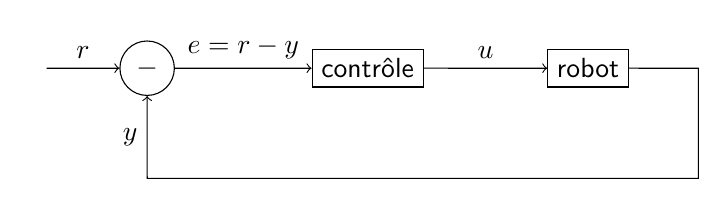
\begin{tikzpicture}[scale=1.4]
\node (input) at (0,1) {};
\node[circle,draw] (diff) at (1,1) {$-$};
\node[rectangle,draw] (control) at (3,1) {\textsf{contrôle}};
\node[rectangle,draw] (robot) at (5,1) {\textsf{robot}};
\draw[->] (input) -- node[above] {$r$} (diff);
\draw[->] (diff)  -- node[above] {$e=r-y$} (control);
\draw[->] (control) -- node[above] {$u$} (robot);
\draw[->] (robot) -- ++(1,0) -- ++(0,-1) -- ++(-5,0) -- node[left] {$y$} (diff);
\end{tikzpicture}
\caption{Un système de contrôle en boucle fermée}\label{fig.control-model}
\end{center}
\end{figure}

Le modèle de la Fig. \ref{fig.control-model} est également appelé un \emph{système de contrôle à rétroaction} car la valeur de sortie $y$ est renvoyée à l'algorithme de contrôle et utilisée pour calculer la valeur de contrôle. La sortie est comparée à la valeur de référence pour calculer $e=r-y$, l'\emph{erreur}. L'algorithme de commande utilise l'erreur pour générer le signal de commande $u$ qui constitue l'entrée du robot.

\subsection{La période d'un algorithme de contrôle}
\index{Période de l'algorithme de contrôle}

Les algorithmes de contrôle sont exécutés périodiquement (Algorithme~\ref{alg.control-loop}). Le logiciel du robot initialise une \emph{variable de temporisation} à la durée requise de la période d'exécution de l'algorithme, par exemple, toutes les $20$ ms. L'ordinateur embarqué possède une \emph{horloge matérielle} qui ``saute'' à intervalles fixes, provoquant une interruption. L'interruption est gérée par le système d'exploitation qui décrémente la valeur de la variable timer. Lorsque la valeur de cette variable atteint zéro, la minuterie a expiré et un événement est déclenché dans le logiciel, ce qui entraîne l'exécution de l'algorithme de contrôle.

\begin{figure}
\begin{alg}{Schéma de l'algorithme de contrôle}{control-loop}
\hline
\hline
&\idv{}integer period&// Duration of timer period\\
&\idv{}integer timer&// Timer variable\\
\hline
\stl{}&period \ass $\cdots$&// Period in milliseconds\\
\stl{}&timer \ass period&// Initialize the timer\\
\stl{}&loop&\\
\stl{}&\idc{}when timer-expired-event occurs&\\
\stl{}&\idc{}\idc{}control algorithm&// Run the algorithm\\
\stl{}&\idc{}\idc{}timer \ass period&// Reset the timer\\
\hline\hline
&// {\bfseries Operating system}&\\
\stl{}&when hardware-clock-interrupt occurs&\\
\stl{}&\idc{} timer \ass timer $-$ $1$&// Decrement the timer\\
\stl{}&\idc{} if timer $=$ $0$&// If the timer expires\\
\stl{}&\idc{}\idc{} raise timer-expired-event&// \ \ \ \ raise an event\\
\end{alg}
\end{figure}

La période de l'algorithme est un paramètre important dans la conception d'un système de contrôle. Si la période est trop courte, de précieuses ressources informatiques seront gaspillées et l'ordinateur peut être surchargé au point que les commandes au robot arrivent trop tard. Si la période est trop longue, le robot ne pourra pas réagir à temps pour corriger les erreurs de son mouvement.

\medskip

\noindent\textbf{Exemple} Considérons un robot qui s'approche d'un objet situé à $10$ cm à une vitesse de $2$ cm/s. Une période de commande de $1$ ms entraînerait un gaspillage de ressources informatiques car le robot ne se déplacera que de $0,002$ cm ($0,02$ mm) pendant chaque cycle de $1$ ms de l'algorithme de commande. Les variations de la puissance du moteur sur de si petites distances n'affecteront pas la capacité du robot à accomplir sa tâche. À l'extrême opposé, une période de contrôle de $2$ s est encore pire : le robot se déplacera de $4$ cm pendant cette période et risque de s'écraser sur l'objet. Une période de contrôle d'environ $0,25$ s ($250$ ms) pendant laquelle le robot se déplace de $0,5$ cm semble une valeur raisonnable pour commencer, car $0,5$ cm est une distance significative en termes d'approche d'un objet. Vous pouvez expérimenter des périodes autour de cette valeur pour déterminer la période optimale : celle qui permet d'obtenir un comportement satisfaisant avec une période aussi longue que possible pour réduire le coût du calcul.

\begin{framed}
\act{Définir la période de contrôle}{Setperiod}
\begin{itemize}
\item Dans l'exemple, nous sommes arrivés à la conclusion que la période optimale de l'algorithme de contrôle était de l'ordre de grandeur des dixièmes de seconde. Dans cette activité, nous vous demandons de réfléchir à ce que devrait être la période optimale pour d'autres algorithmes de contrôle.
\item Un système de chauffage domestique contient un thermostat pour contrôler la température. Quelle serait la période optimale pour l'algorithme de contrôle ? La période dépend des paramètres techniques du système de chauffage et des propriétés physiques de la transmission de la chaleur dans les pièces. Expliquez comment vous mesureriez ces facteurs et comment ils affectent la période de contrôle.
\item Considérez une voiture autonome qui essaie de se garer. Quelles hypothèses devez-vous formuler pour concevoir une période de contrôle ? Quelle serait une période raisonnable ?
\item Comment les propriétés des capteurs affectent-elles la période de contrôle ? Dans l'exemple d'un robot qui s'approche d'un objet, comment la période change-t-elle si le capteur peut détecter l'objet à $2$ cm, $5$ cm, $10$ cm, $20$ cm, $40$ cm ?
\end{itemize}
\end{framed}

%\section{Agorithmes de contrôle}\label{s.control-alg}
\index{algorithme!control}

Nous définissons maintenant une séquence de quatre algorithmes de contrôle, chacun s'appuyant sur le précédent et fournissant un contrôle plus précis, au prix d'une plus grande complexité de calcul. En pratique, le concepteur du système doit choisir l'algorithme le plus simple qui permet au robot de remplir sa tâche.

Les algorithmes sont présentés dans le contexte d'un robot qui doit s'approcher d'un objet et s'arrêter à une distance $s$ devant celui-ci. La distance est mesurée par un capteur de proximité et la vitesse du robot est contrôlée en réglant la puissance des moteurs.

\section{Contrôle on-off}\label{s.on-off}
\index{Algorithme!control-on-off}

Le premier algorithme de contrôle est appelé l'algorithme \emph{on-off} ou \emph{bang-bang} (Algorithme~\ref{alg.onoff}). On définit une constante \p{référence} qui est la distance devant l'objet à laquelle le robot doit s'arrêter. La variable \p{mesured} est la distance réelle mesurée par le capteur de proximité. La variable \p{error} est la différence entre les deux :
\begin{center}
\p{erreur} $\leftarrow$ \p{référence} $-$ \p{mesuré},
\end{center}
qui est négatif si le robot est trop éloigné de l'objet et positif s'il est trop proche de l'objet. Les puissances des moteurs sont tournées à fond en avant ou à fond en arrière selon le signe de l'erreur. Par exemple, si la distance de référence est de $10$ cm et la distance mesurée de $20$ cm, le robot est trop éloigné et l'erreur est de $10$ cm. Par conséquent, les moteurs doivent être réglés pour se déplacer vers l'avant.

\begin{figure}
\begin{alg}{Contrôleur désactivé}{onoff}
&\idv{}integer reference \ass $\cdots$&// Reference distance\\
&\idv{}integer measured &// Measured distance\\
&\idv{}integer error &// Distance error\\
\hline
\stl{}&error \ass reference $-$ measured&\\
\stl{}&if error $<$ 0&\\
\stl{}&\idc{} left-motor-power \ass $100$&// Move forwards\\
\stl{}&\idc{} right-motor-power \ass $100$&\\
\stl{}&if error $=$ 0&\\
\stl{}&\idc{} left-motor-power \ass $0$&// Turn off motors\\
\stl{}&\idc{} right-motor-power \ass $0$&\\
\stl{}&if error $>$ 0&\\
\stl{}&\idc{} left-motor-power \ass $-100$&// Move backwards\\
\stl{}&\idc{} right-motor-power \ass $-100$&\\
\end{alg}
\end{figure}

Le robot s'approche de l'objet à pleine vitesse. Lorsque le robot atteint la distance de référence par rapport à l'objet, il faut du temps pour que le capteur soit lu et que l'erreur soit calculée. Même si le robot mesure une distance exactement égale à la distance de référence (ce qui est peu probable), le robot ne pourra pas s'arrêter immédiatement et dépassera la distance de référence. L'algorithme fait alors reculer le robot à pleine vitesse, en dépassant à nouveau la distance de référence. Lorsque la minuterie déclenche une nouvelle exécution de l'algorithme de contrôle, le robot inverse sa direction et avance à pleine vitesse. Le comportement du robot est illustré à la Fig.\ref{fig.onoff} : le robot oscille autour de la distance de référence par rapport à l'objet. Il est très peu probable que le robot s'arrête réellement à la distance de référence ou à proximité.

\begin{figure}
\begin{center}
\begin{tikzpicture}[scale=1.2]
\draw[<->] (0,5) -- node[sloped,above,rotate=180] {\p{distance}} (0,0) node[left] {} -- node[below] {\p{temps}} (8,0);
\draw (0,2) node[below right] {$r$} -- (8,2);
\draw[thick] plot coordinates {(0,5) (2,1.5) (3,2.5) (4,1.5) (5,2.5) (6,1.5)(7,2.5) (8,1.5)};
\end{tikzpicture}
\caption{Comportement de l'algorithme on-off}\label{fig.onoff}
\end{center}
\end{figure}

Un autre inconvénient de l'algorithme on-off est que l'inversion fréquente et brutale de la direction entraîne des accélérations élevées. Si l'on essaie de contrôler un bras de préhension, les objets qu'il porte peuvent être endommagés. L'algorithme génère des niveaux élevés d'usure des moteurs et des autres pièces mécaniques mobiles.

\begin{framed}
\act{Contrôleur désactivé}{onoff}
\begin{itemize}
\item Implémentez l'algorithme on-off sur votre robot pour la tâche consistant à s'arrêter à une distance de référence d'un objet.
\item Exécutez-le plusieurs fois en commençant à des distances différentes de l'objet.
\item L'algorithme~\ref{alg.onoff} arrête le robot lorsque l'erreur est exactement nulle. Modifiez l'implémentation pour que le robot s'arrête si l'erreur est comprise dans une petite plage autour de zéro. Expérimentez différentes plages et voyez comment elles affectent le comportement du robot.
\end{itemize}
\end{framed}

\section{Contrôleur proportionnel (P)}\label{s.p}
\index{controler!algorithme!proportionnel}

Pour développer un meilleur algorithme, nous nous inspirons de la conduite d'un vélo. Supposons que vous êtes en train de rouler à vélo et que vous voyez que le feu de circulation devant vous est passé au rouge. Vous n'attendez pas le dernier moment, lorsque vous êtes sur la ligne d'arrêt, pour appuyer à fond sur le levier de frein ; si vous le faites, vous risquez d'être éjecté de votre vélo ! Ce que tu fais, c'est de ralentir progressivement ta vitesse : d'abord, tu arrêtes de pédaler ; ensuite, tu serres doucement le frein pour ralentir un peu plus ; enfin, quand tu es sur la ligne d'arrêt et que tu vas lentement, tu serres plus fort pour arrêter complètement le vélo. L'algorithme utilisé par un cycliste peut être exprimé comme suit :
\begin{quote}
\normalsize\noindent{}Réduisez davantage votre vitesse à mesure que vous vous rapprochez de la distance de référence.
\end{quote}
La diminution de la vitesse est (inversement) \emph{proportionnelle} à la proximité du feu : plus vous êtes proche, plus vous ralentissez. Le facteur de proportionnalité est appelé le \emph{gain}\index{gain} de l'algorithme de contrôle. Une autre façon d'exprimer cet algorithme est la suivante :
\begin{quote}
\normalsize\noindent{}Réduisez votre vitesse au fur et à mesure que l'erreur entre la distance de référence et la distance mesurée diminue.
\end{quote}

Algorithme~\ref{alg.proportionnel} est l'\emph{algorithme de contrôle proportionnel} ou un \emph{contrôleur P}.

\begin{figure}
\begin{alg}{Contrôleur proportionnel}{proportionnel}
&\idv{}integer reference \ass $\cdots$&// Reference distance\\
&\idv{}integer measured &// Measured distance\\
&\idv{}integer error &// Error\\
&\idv{}float gain \ass $\cdots$& // Proportional gain\\
&\idv{}integer power & // Motor power\\
\hline
\stl{}&error \ass reference $-$ measured&// Distances\\
\stl{}&power \ass gain * error&// Control value\\
\stl{}&left-motor-power \ass power&\\
\stl{}&right-motor-power \ass power&\\
\end{alg}
\end{figure}

\medskip

\noindent\textbf{Exemple} Supposons que la distance de référence soit de $100$ cm et que le gain soit de $-0.8$. Lorsque le robot se trouve à $150$ cm de l'objet, l'erreur est de $100-150=-50$ et l'algorithme de contrôle fixera la puissance à
$-0.8\cdot -50=40$. Le tableau~\ref{tab.p-controller} présente les erreurs et les réglages de puissance pour trois distances. Si le robot dépasse la distance de référence de $100$ cm et qu'une distance de $60$ cm est mesurée, la puissance sera réglée sur $-32$, ce qui entraînera un recul du robot.

\begin{table}
\caption{Contrôleur proportionnel pour un gain de $-0.8$}
\label{tab.p-controller}
\begin{tabular}{rrr}
\hline
\multicolumn{1}{c}{distance} & \multicolumn{1}{c}{erreur}& \multicolumn{1}{c}{puissance}\\\hline
$150$ & $-50$ & $40$\\
$125$ & $-25$ & $20$\\
$60$ & $40$ & $-32$\\
\hline
\end{tabular}
\end{table}

La figure~\ref{fig.p-control} représente la distance du robot à l'objet en fonction du temps lorsque le robot est contrôlé par un contrôleur P. La ligne étiquetée $r$ représente la distance de référence. La variation de la puissance du moteur est régulière et le robot ne subit pas d'accélérations et de décélérations rapides. La réponse est un peu lente, mais le robot se rapproche de la distance cible.

\begin{figure}
\begin{center}
\begin{tikzpicture}[scale=1.2]
\draw[<->] (0,5) -- node[sloped,above,rotate=180] {\p{distance}} (0,0) node[left] {} -- node[below] {\p{temps}} (8,0);
\draw (0,1.9) node[below right] {$r$} -- (8,1.9);
\draw[domain=0:8,samples=100,thick] plot (\x,{3*exp(-2*\x)+2});
\end{tikzpicture}
\caption{Comportement du contrôleur P}\label{fig.p-control}
\end{center}
\end{figure}

Malheureusement, le robot n'atteint pas réellement la distance de référence. Pour comprendre pourquoi cela se produit, considérez ce qui se passe lorsque le robot est très proche de la distance de référence. L'erreur sera très faible et, par conséquent, le réglage de la puissance sera très bas. En théorie, le faible réglage de la puissance doit permettre au robot de se déplacer lentement, pour finalement atteindre la distance de référence. En pratique, la puissance du moteur peut devenir si faible qu'elle ne parvient pas à surmonter la friction interne des moteurs et de leur connexion aux roues, et le robot s'arrête alors de bouger.

Il pourrait sembler que l'augmentation du gain du contrôleur P pourrait surmonter ce problème, mais un gain élevé souffre d'un sérieux inconvénient. La figure~\ref{fig.gain} montre l'effet du gain du contrôleur P. Un gain plus élevé (ligne rouge en pointillés) permet au robot de se rapprocher plus rapidement de la distance de référence, tandis qu'un gain plus faible (ligne bleue en pointillés) permet au robot de se rapprocher plus lentement de la distance de référence. Cependant, si le gain est trop élevé, le contrôleur P fonctionne comme un contrôleur tout ou rien avec une réponse oscillante (ligne verte). Nous disons que le contrôleur est \emph{instable}.

\begin{figure}
\begin{center}
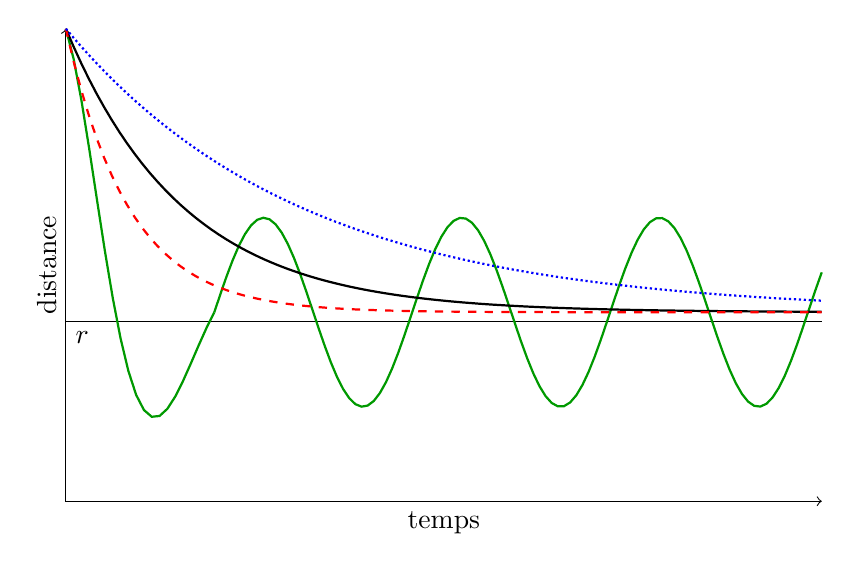
\begin{tikzpicture}[scale=1.2]
\draw[<->] (0,5) -- node[sloped,above,rotate=180] {\p{distance}} (0,0) node[left] {} -- node[below] {\p{temps}} (8,0);
\draw (0,1.9) node[below right] {$r$} -- (8,1.9);
\draw[domain=0:1.57,samples=20,thick,green!60!black] plot (\x,{3*exp(-\x)*cos(3*\x r)+2});
\draw[domain=1.57:8,samples=100,thick,green!60!black] plot (\x,{cos(3*\x r)+2});
\draw[domain=0:8,samples=100,thick] plot (\x,{3*exp(-.8*\x)+2});
\draw[domain=0:8,samples=100,dashed,red,thick] plot (\x,{3*exp(-1.5*\x)+2});
\draw[domain=0:8,samples=100,densely dotted,blue,thick] plot (\x,{3*exp(-.4*\x)+2});
\end{tikzpicture}
\caption{L'effet du gain sur le régulateur P : gain faible (ligne bleue pointillée), gain élevé (ligne rouge pointillée), gain excessif (ligne verte oscillante)}\label{fig.gain}
\end{center}
\end{figure}

Il existe des situations où le contrôleur P ne peut pas atteindre la distance de référence, même dans un système idéal. Supposons que l'objet lui-même s'éloigne du robot à vitesse constante. Le contrôleur P règle la puissance maximale du moteur pour que le robot se déplace rapidement vers l'objet. Cependant, à mesure que le robot s'approche de l'objet, la distance mesurée devient faible et le contrôleur P règle la puissance à un niveau si bas que la vitesse du robot est inférieure à celle de l'objet. En conséquence, le robot n'atteindra jamais la distance de référence. Si le robot pouvait effectivement atteindre la distance de référence, l'erreur serait nulle et la vitesse du robot serait donc également nulle. Cependant, l'objet continue de s'éloigner du robot, de sorte que, un peu plus tard, le robot recommence à se déplacer et le cycle se répète. Ce mouvement de va-et-vient n'est pas l'objectif visé par le maintien de la distance de référence.

\smallskip

\noindent\textbf{Exemple} Nous utilisons les mêmes données que dans l'exemple précédent, sauf que l'objet se déplace à $20$ cm/s. Le tableau~\ref{tab.p-controller-moving} montre les erreurs et les réglages de puissance pour trois distances. Au départ, le robot va plus vite que l'objet, il va donc le rattraper. Cependant, à $125$ cm de l'objet, le robot se déplace à la même vitesse que l'objet. Il maintient cette distance fixe et ne se rapprochera pas de la distance de référence de $100$ cm. Si, d'une manière ou d'une autre, le robot se rapproche de l'objet, disons à $110$ cm, la puissance est réduite à $8$, ce qui fait que le robot s'éloigne de l'objet.

\begin{table}
\caption{Contrôleur proportionnel pour un objet en mouvement et un gain de $-0.8$}
\label{tab.p-controller-moving}
\begin{tabular}{rrr}
\hline
\multicolumn{1}{c}{distance} & \multicolumn{1}{c}{erreur}& \multicolumn{1}{c}{puissance}\\
\hline
$150$ & $-50$ & $40$\\
$125$ & $-25$ & $20$\\
$110$ & $-10$ & $8$\\
\hline
\end{tabular}
\end{table}

En général, le robot se stabilise à une distance fixe de la distance de référence. Vous pouvez réduire cette erreur en augmentant le gain, mais la distance de référence ne sera jamais atteinte et le seul résultat est que le contrôleur devient instable.

\begin{framed}
\act{Régulateur proportionnel}{proportional}
\begin{itemize}
\item Mettez en œuvre l'algorithme de contrôle proportionnel pour que le robot s'arrête à une distance donnée d'un objet. Avec quelle précision pouvez-vous atteindre l'objectif lorsque l'objet ne bouge pas ?
\item Que se passe-t-il si l'objet bouge ? Pour l'objet, vous pouvez utiliser un second robot programmé pour se déplacer à une vitesse fixe.
\item Expérimentez avec le gain et la période pour voir comment ils affectent les performances de l'algorithme.
\end{itemize}
\end{framed}

\section{Contrôleur proportionnel-intégral (PI)}\label{s.pi}
\index{Contrôleur!algorithme!proportionnel-intégral}

Un \emph{contrôleur proportionnel-intégral} peut atteindre la distance de référence même en présence de friction ou d'un objet en mouvement en prenant en compte l'erreur accumulée au fil du temps. Alors que le contrôleur P ne prend en compte que l'erreur courante :
\[
u(t) = k_pe(t)\,,
\]
le contrôleur PI ajoute l'intégrale de l'erreur depuis le moment où l'algorithme commence à fonctionner jusqu'au moment présent :
\[
u(t) = k_pe(t) + k_i\int_{0}^t e(\tau)\,d\tau\,.
\]
Des facteurs de gain distincts sont utilisés pour les termes proportionnels et intégraux afin de permettre une certaine souplesse dans la conception du contrôleur.

Lors de la mise en œuvre d'un régulateur PI, une approximation discrète de l'intégrale continue est effectuée (Algorithme~\ref{alg.pi-controller}).

\begin{figure}
\begin{alg}{Contrôleur proportionnel-intégral}{pi-controller}
&\idv{}integer reference \ass $\cdots$&// Reference distance\\
&\idv{}integer measured &// Measured distance\\
&\idv{}integer error &// Error\\
&\idv{}integer error-sum $\leftarrow 0$&// Cumulative error\\
&\idv{}float gain-p \ass $\cdots$& // Proportional gain\\
&\idv{}float gain-i \ass $\cdots$& // Integral gain\\
&\idv{}integer power & // Motor power\\
\hline
\stl{}&error \ass reference $-$ measured&// Distances\\
\stl{}&error-sum \ass error-sum + error&// Integral term\\
\stl{}&power \ass gain-p * error + gain-i * error-sum&// Control value\\ 
\stl{}&left-motor-power \ass power&\\
\stl{}&right-motor-power \ass power&\\
\end{alg}
\end{figure}

En présence d'un frottement ou d'un objet en mouvement, l'erreur sera intégrée et entraînera le réglage d'une puissance moteur plus élevée, ce qui permettra au robot de converger vers la distance de référence. Un problème avec un contrôleur PI est que l'intégration de l'erreur commence à l'état initial lorsque le robot est éloigné de l'objet. Lorsque le robot s'approche de la distance de référence, le terme intégral du régulateur aura déjà une valeur importante ; pour diminuer cette valeur, le robot doit se déplacer au-delà de la distance de référence de manière à obtenir des erreurs de signe opposé. Cela peut générer des oscillations (Fig.~\ref{fig.pi-control}).

\begin{figure}
\begin{center}
\begin{tikzpicture}[scale=1.2]
\draw[<->] (0,5) -- node[sloped,above,rotate=180] {\p{distance}} (0,0) node[left] {} -- node[below] {\p{temps}} (8,0);
\draw (0,2) node[below right,xshift=-1pt] {$r$} -- (8,2);
\draw[domain=0:8,samples=100,thick] plot (\x,{3*exp(-1*\x)*cos(5*\x r)+2});
\end{tikzpicture}
\caption{Comportement du contrôleur PI}\label{fig.pi-control}
\end{center}
\end{figure}

\begin{framed}
\act{Contrôleur PI}{Contrôleur PI}
\begin{itemize}
\item Implémentez un contrôleur PI qui oblige le robot à s'arrêter à une distance donnée d'un objet.
\item Comparez le comportement du contrôleur PI à celui d'un contrôleur P pour la même tâche en surveillant les variables des algorithmes de contrôle dans le temps.
\item Que se passe-t-il si vous empêchez manuellement le robot de bouger pendant un court instant, puis que vous le laissez partir ? Cela illustre un concept appelé \emph{intégrator windup}\index{control!integrator windup}. Explorez ce concept en consultant des sources en ligne et trouvez une méthode pour résoudre le problème.
\end{itemize}
\end{framed}

\section{Contrôleur proportionnel-intégral-dérivé (PID)}\label{s.pid}
\index{Contrôleur!algorithme!proportionnel-intégral-derivé}

Lorsque vous lancez ou bottez un ballon vers un autre joueur qui se déplace, vous ne le lancez pas vers sa position actuelle. Le temps que le ballon l'atteigne, il se sera déplacé vers une nouvelle position. Au lieu de cela, vous estimez l'endroit où se trouvera la nouvelle position et vous y dirigez la balle. De même, un robot dont la tâche consiste à pousser un colis sur un chariot en mouvement doit synchroniser sa poussée avec la position future estimée du chariot lorsque le colis l'atteint. L'algorithme de commande de ce robot ne peut pas être un contrôleur tout-ou-rien, P ou PI, car ils ne prennent en compte que la valeur actuelle de l'erreur (et pour le contrôleur PI, les valeurs précédentes). 

Pour estimer l'erreur future, le taux de variation de l'erreur peut être pris en compte. Si le taux de variation de l'erreur est faible, le robot peut pousser le colis juste avant que le chariot ne s'en approche, tandis que si le taux de variation de l'erreur est élevé, le colis doit être poussé beaucoup plus tôt.

Mathématiquement, le taux de variation est exprimé sous la forme d'une dérivée. Un régulateur \emph{proportionnel-intégral-dérivé (PID)} ajoute un terme supplémentaire aux termes P et I :
\begin{equation}
u(t) = k_pe(t) + k_i\int_{\tau=0}^t e(\tau)\,d\tau + k_d \frac{de(t)}{dt}\,.\label{eq.pid}
\end{equation}

Dans la mise en œuvre d'un contrôleur PID, le différentiel est approximé par la différence entre l'erreur précédente et l'erreur actuelle (Algorithme~\ref{alg.pid-controller}).

\begin{figure}
\begin{alg}{Contrôleur proportionnel-intégral-différentiel}{pid-controller}
&\idv{}integer reference \ass $\cdots$&// Reference distance\\
&\idv{}integer measured &// Measured distance\\
&\idv{}integer error &// Error\\
&\idv{}integer error-sum $\leftarrow 0$ &// Cumulative error\\
&\idv{}integer previous-error \ass 0&// Previous error\\
&\idv{}integer error-diff &// Error difference\\
&\idv{}float gain-p \ass $\cdots$& // Proportional gain\\
&\idv{}float gain-i \ass $\cdots$& // Integral gain\\
&\idv{}float gain-d \ass $\cdots$& // Derivative gain\\
&\idv{}integer power & // Motor power\\
\hline
\stl{}&error \ass reference $-$ measured&// Distances\\
\stl{}&error-sum \ass error-sum + error&// Integral term\\
\stl{}&error-diff \ass error $-$ previous-error&// Differential term\\
\stl{}&previous-error \ass error&// Save current error\\
\stl{}&power \ass gain-p * error + &// Control value\\ 
&\idc{}gain-i * error-sum + gain-d * error-diff&\\ 
\stl{}&left-motor-power \ass power&\\
\stl{}&right-motor-power \ass power&\\
\end{alg}
\end{figure}

Le comportement du contrôleur PID est illustré sur la Fig.\ref{fig.pid-control}. Le robot converge rapidement et en douceur vers la distance de référence. 

\begin{figure}
\begin{center}
\begin{tikzpicture}[scale=1.2]
\draw[<->] (0,5) -- node[sloped,above,rotate=180] {\p{distance}} (0,0) node[left] {} -- node[below] {\p{temps}} (8,0);
\draw[dashed] (0,2) node[below right] {$r$} -- (8,2);
\draw[domain=0:8,samples=100,thick] plot (\x,{2.5*exp(-2*\x)+2});
\end{tikzpicture}
\caption{Comportement du contrôleur PID}\label{fig.pid-control}
\end{center}
\end{figure}

Les gains d'un régulateur PID doivent être soigneusement équilibrés. Si les gains des termes P et I sont trop élevés, des oscillations peuvent se produire. Si le gain du terme D est trop élevé, le régulateur réagira à de courtes salves de bruit.


\begin{framed}
\act{Contrôleur PID}{Contrôleur PID}
\begin{itemize}
\item Implémentez un contrôleur PID pour la tâche d'un robot s'approchant d'un objet.
\item Expérimentez avec différents gains jusqu'à ce que le robot se rapproche en douceur de la distance de référence.
\item Répétez les expériences avec un objet en mouvement.
\end{itemize}
\end{framed}

\section{Résumé}

Un bon algorithme de contrôle doit converger rapidement vers le résultat souhaité tout en
tout en évitant les mouvements brusques. Il doit être efficace en termes de calcul, mais ne pas nécessiter de réglage constant. L'algorithme de contrôle doit être adapté aux exigences spécifiques du système et de la tâche, et fonctionner correctement dans différentes conditions environnementales. Nous avons décrit quatre algorithmes, de l'impraticable algorithme tout ou rien à des algorithmes combinant des termes proportionnels, intégraux et dérivés. Le terme proportionnel garantit que les erreurs importantes entraînent une convergence rapide vers la référence, le terme intégral garantit que la référence peut effectivement être atteinte, tandis que le terme dérivé rend l'algorithme plus réactif. 

\section{Lectures complémentaires}

Un manuel moderne sur les algorithmes de contrôle est \cite{astrom-murray}.

